% !TEX program = xelatex

\documentclass[12pt,a4paper]{article}
\usepackage[UTF8]{ctex}
\usepackage{float}
\usepackage{amsmath}
\usepackage{enumerate}
\usepackage{booktabs}
\usepackage{graphicx}
\usepackage{longtable}
\usepackage{subfigure}

\usepackage{url}
\usepackage{multirow}

% for plotting 
\usepackage{caption}
\usepackage{pgfplots}

% for pseudo code 
\usepackage{algorithm}
\usepackage[noend]{algpseudocode}

% for reference 
\usepackage{hyperref}
\usepackage{cleveref}

% for code 
\usepackage{listings}
\usepackage{xcolor}
\usepackage{fontspec}
\definecolor{darkgreen}{rgb}{0,0.6,0}
\newfontfamily\consolas{Consolas}

\lstset {
    basicstyle=\footnotesize\consolas, % basic font setting
    breaklines=true, 
    frame=single,     % {single, shadowbox, bottomline}
    keywordstyle=\color{blue}, 
    commentstyle=\color{darkgreen},
    stringstyle=\color{red},
    showstringspaces=false,
    % backgroundcolor=\color{black!5}, % set backgroundcolor
    numbers=left, 
    numberstyle=\ttfamily,
}

% Microsoft Word A4 paper default layout 
\usepackage[a4paper, left=3.18cm, right=3.18cm, top=2.54cm, bottom=2.54cm]{geometry}

% \captionsetup[figure]{labelfont={bf}, name={Figure}}
% \captionsetup[table]{labelfont={bf}, name={Table}}

\crefname{equation}{方程}{方程}
\Crefname{equation}{方程}{方程}
\crefname{table}{表}{表}
\Crefname{table}{表}{表}
\crefname{figure}{图}{图}
\Crefname{figure}{图}{图}

\title{数学实验:第一次作业}
\author{计算机系 \quad 计73 \quad 2017011620 \quad 李家昊}
\date{\today}

% 实验报告格式的基本要求

% 系别、班级、学号、姓名

% 1 实验目的
% 2 题目
%   2.1 计算题:题号,算法设计(包括计算公式),程序,计算结果(计算机输出),结果分析,结论。
%   2.2 应用题:题号,问题分析,模型假设,模型建立,算法设计(包括计算公式),程序,计算结果(计算机输出),结果的数学分析,结果的实际意义,结论。
% 3 收获与建议

\begin{document}

\maketitle

\section{实验目的}

\begin{itemize}
    \item 掌握用MATLAB计算拉格朗日、分段线性、三次样条三种插值的方法,改变节点的数目,对三种插值结果进行初步分析。
    \item 掌握用MATLAB及梯形公式、辛普森公式计算数值积分。
    \item 通过实例学习用插值和数值积分解决实际问题。
\end{itemize}

\section{问题求解}

\subsection{Chap3-Ex5 (Calc)}

\subsubsection{算法设计}

本题要求选用三种数值积分方法计算$\pi$。

首先需要选择合适的定积分公式来计算$\pi$,为了计算的简单起见,选择公式如下,
\begin{equation}
    \pi = 4 \int_0^1 \sqrt{1 - x^2} dx
\end{equation}
被积函数是单位圆在第一象限的函数图象,不含复杂运算,计算速度相对较快。我们只需要用数值积分的方法计算出右端的定积分,就可以确定$\pi$的近似值。

这里采用上课时介绍的三种数值积分方法来计算定积分,分别为梯形公式,辛普森公式,以及Gauss-Lobatto公式。

\subsubsection{Matlab程序}

Matlab程序如下,为了统计出不同误差限下的近似计算次数,这里写了一个简单的二分查找,详见代码,
\lstinputlisting[language=Matlab]{../src/ex5.m}

\subsubsection{计算结果}

在不同误差限下的计算结果和计算次数如\Cref{tab:ex5_pi}所示。

\begin{table}
    \centering
    \caption{三种积分公式在不同误差限下的计算结果及计算次数。}
    \label{tab:ex5_pi}
    \begin{tabular}{c|c|ccccc}
        \toprule
        \multicolumn{2}{c|}{绝对误差限} & 1e-6 & 1e-8 & 1e-10\tabularnewline
        \midrule
        \multirow{2}{*}{梯形公式} & 数值 & 3.141591653694 & 3.141592643590 &
        3.141592653490\tabularnewline
        & 次数 & 11143 & 240032 & 5171199\tabularnewline
        \hline
        \multirow{2}{*}{辛普森公式} & 数值 & 3.141591970545 & 3.141592649744 &
        3.141592653419\tabularnewline
        & 次数 & 73 & 193 & 357\tabularnewline
        \hline
        \multirow{2}{*}{Gauss-Lobatto} & 数值 & 3.141585181550 & 3.141592647723 &
        3.141592653429\tabularnewline
        & 次数 & 78 & 168 & 378\tabularnewline
        \bottomrule
    \end{tabular}
\end{table}

\subsubsection{结果分析}

三种积分算法均可以逼近$\pi$,但在相同计算开销下,梯形公式的精确度最低,辛普森公式和Gauss-Lobatto公式的精确度相近。此外,随着分割粒度的细化,三种算法的精度都有了相应的提升。在实际情况中,往往需要根据精度要求来调整分割粒度。

\subsubsection{结论}

本实验中计算得出的$\pi$的数值为3.141592653429。

\subsection{Chap3-Ex10 (Calc)}

\subsubsection{算法设计}

本题给出了机翼断面轮廓线上稀疏的采样点,需要求出细粒度的断面轮廓以及断面的面积。

给定断面点$\{(x_i, y_i)\}_{i=0}^n$,求插值点 $x$ 处的插值$y$,这里选取三种方式进行插值,分别是拉格朗日插值,分段线性插值,以及三次样条插值。

对于拉格朗日插值,插值多项式为,
\begin{equation}\label{eq:lagrange}
    L(x) = \sum_{i=0}^n y_i l_i(x)
\end{equation}
其中满足,
\begin{equation}
    l_i(x) = \prod_{j \ne i} \frac{x - x_j}{x_i - x_j}, \quad i = 0,1,...,n
\end{equation}

对于分段线性插值,插值多项式经过推导,同样可以表示为形如\Cref{eq:lagrange}的形式,其中,
\begin{equation}
    l_i(x) = 
    \begin{cases}
        \dfrac{x - x_{i-1}}{x_i - x_{i-1}}, & x_{i-1}\le x \le x_i\\
        \dfrac{x - x_{i+1}}{x_{i} - x_{i+1}}, & x_i \le x \le x_{i+1}\\
        0, & \text{otherwise}
    \end{cases}
\end{equation}

对于三次样条插值,插值多项式可表示为,
\begin{equation}
    S(x) = \{s_i(x)=a_i x^3 + b_i x^2 + c_i x + d_i \ |\ x\in [x_{i-1}, x_i], i=1,...,n\}
\end{equation}
其中$a_i, b_i, c_i, d_i$为$4n$个待定系数,由下列$4n$个方程唯一确定,
\begin{equation}
    \begin{cases}
        S(x_i) = y_i, & i=0,1,...,n\\
        s_i^{(k)}(x_i) = s_{i+1}^{(k)}(x_i), & k=0,1,2, \quad i=1,2,...,n-1\\
        S''(x_0) = S''(x_n) = 0, &\\
    \end{cases}
\end{equation}

得到插值结果后,采用梯形积分公式来计算机翼断面的面积即可。

\subsubsection{Matlab程序}

其中,拉格朗日插值算法需要自己实现,我在老师给的样例程序上进行了一定的优化,实现如下,
\lstinputlisting[language=Matlab]{../src/lagrange.m}

分段线性插值用Matlab内置的\texttt{interp1(x, y, xq, 'linear')},三次样条插值采用Matlab内置的\texttt{interp1(x, y, xq, 'spline')},完整程序如下,
\lstinputlisting[language=Matlab]{../src/ex10.m}

\subsubsection{计算结果}

采用三种插值方法所得到的机翼断面曲线如\Cref{fig:ex10_interp}所示。根据断面曲线,采用梯形积分公式计算出断面的面积,如\Cref{tab:ex10_area}所示。

\begin{table}[h]
    \centering
    \caption{三种插值方式所得机翼断面的面积。}
    \label{tab:ex10_area}
    \begin{tabular}[]{c|ccc}
        \toprule
        插值算法 & 拉格朗日插值 & 分段线性插值 & 三次样条插值\tabularnewline
        \midrule
        % \endhead
        面积 & 40.30 & 10.75 & 11.34\tabularnewline
        \bottomrule
    \end{tabular}
\end{table}

\begin{figure}[H]
    \centering
    \subfigure[拉格朗日插值]{
        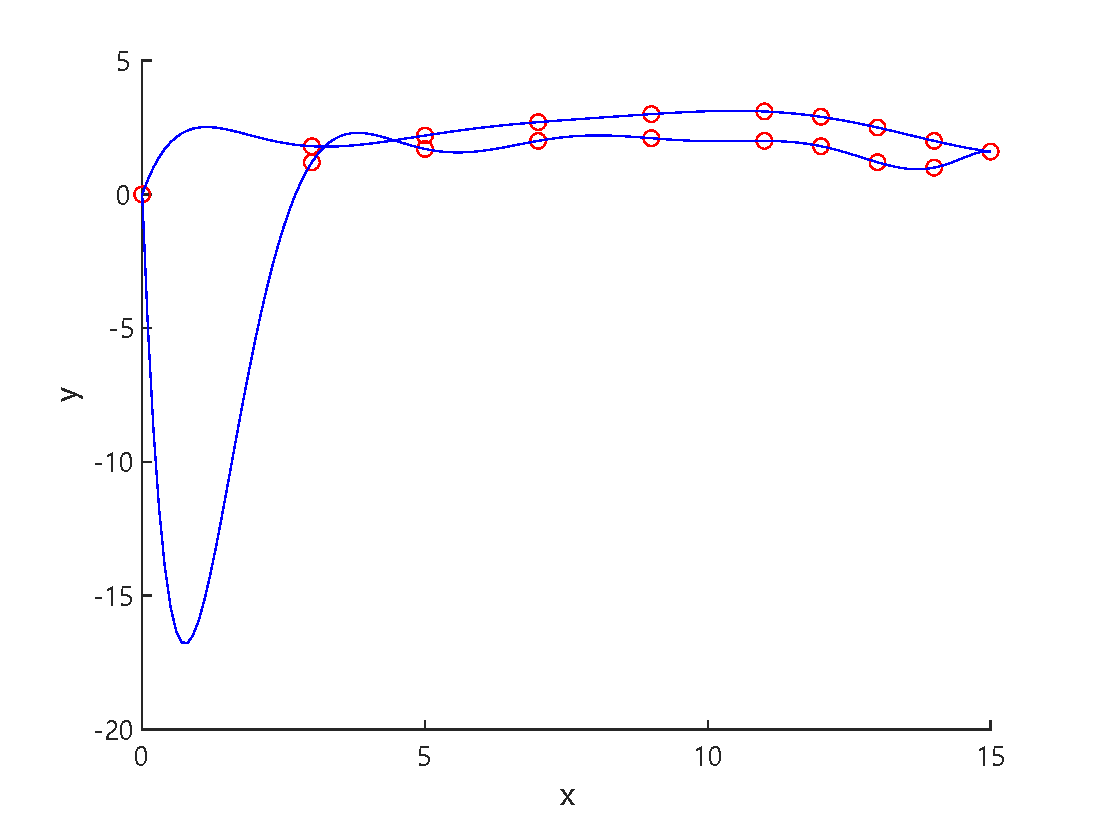
\includegraphics[width=0.6\textwidth]{fig/ex10_lagrange.pdf}
        \label{fig:ex10_lagrange}
    }
    \subfigure[分段线性插值]{
        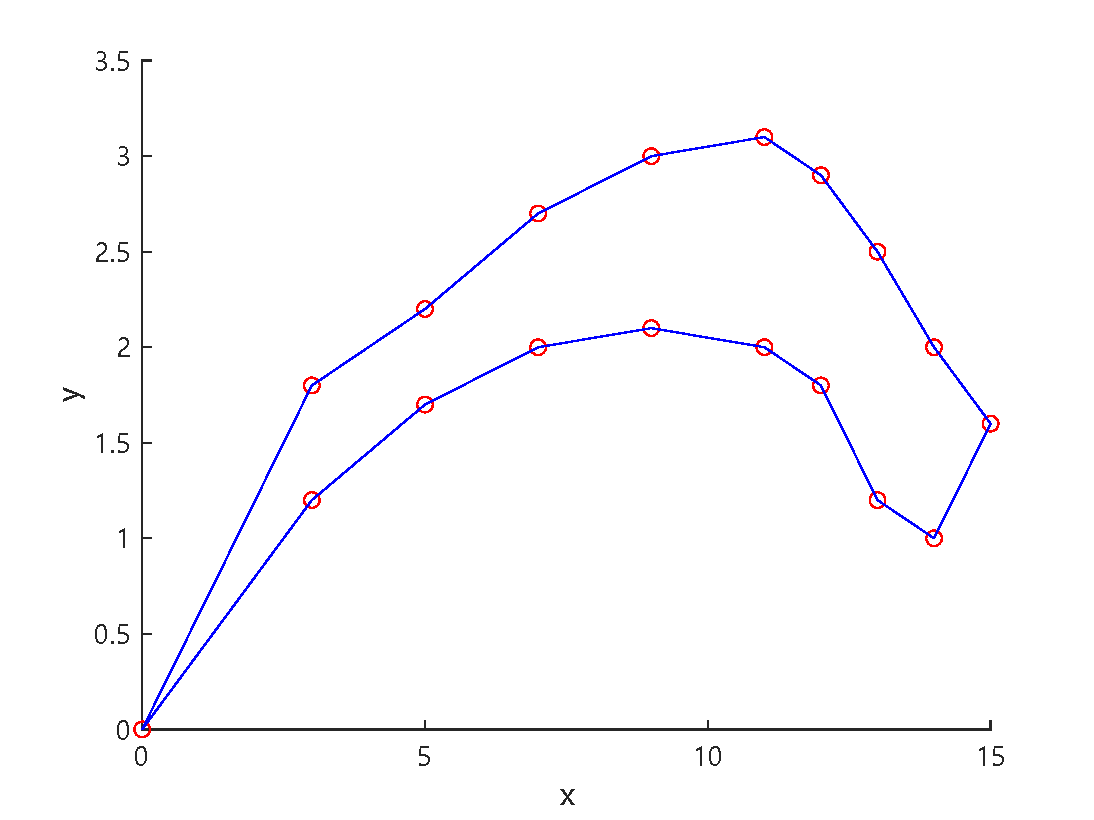
\includegraphics[width=0.6\textwidth]{fig/ex10_linear.pdf}
        \label{fig:ex10_linear}
    }
    \subfigure[三次样条插值]{
        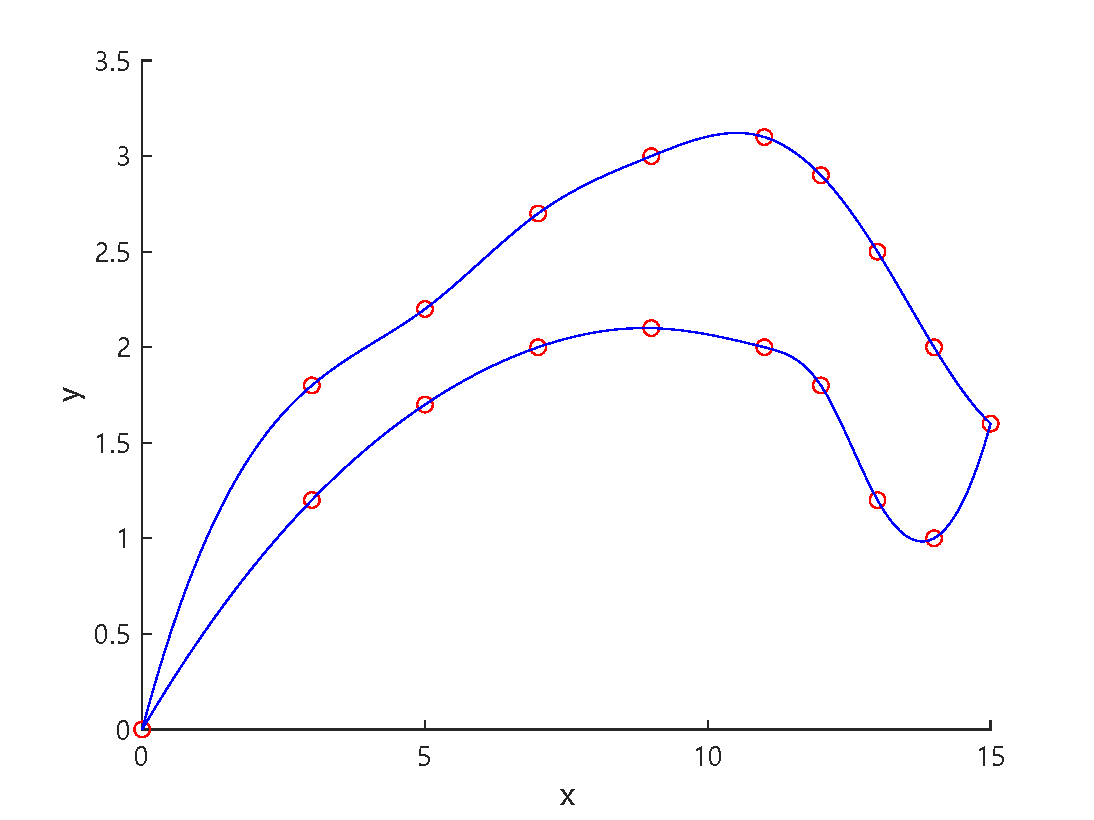
\includegraphics[width=0.6\textwidth]{fig/ex10_spline.pdf}
        \label{fig:ex10_spline}
    }
    \caption{采用三种插值方法得到的断面曲线。}
    \label{fig:ex10_interp}
\end{figure}

\subsubsection{结果分析}

从\Cref{fig:ex10_interp}可以看出,采用拉格朗日插值时,出现了Runge现象,插值曲线振荡强烈,导致的面积计算偏差过大,不能作为实际生产数据使用。采用分段线性插值时,曲线更加平缓,然而在采样点处会出现不光滑的导数不连续点,不利于实际使用。采用三次样条插值时,除了左右端点的结合处,曲线在其他位置均有二阶连续可导的光滑程度,形成的流线有利于降低机翼阻力。

因此,在实际生产中,应当使用三次样条插值所得的曲线和面积结果。

\subsubsection{结论}

实际生产中,应当采用三次样条插值所得的断面曲线,如\Cref{fig:ex10_spline}所示,断面面积为11.34。

\subsection{Chap3-Ex12 (App)}

\subsubsection{问题分析}

题目给出了在几个时刻统计出的一分钟车流量,要求估计一天的车流量。题目给出的信息是很粗糙的,需要首先通过插值估计出一天内每一时刻的一分钟车流量,再进行数值积分求出全天的总车流量。

\subsubsection{模型假设}

考虑到实际情况,这里给出以下假设,
\begin{enumerate}[A.]
    \item 每分钟车流量是非负的
    \item 每分钟车流量随时间的变化是连续的
    \item 每分钟车流量随时间的变化是一阶光滑的
\end{enumerate}

\subsubsection{模型建立}

从一天的零点开始,设经过$t$分钟后$(0\le t \le 1440)$,在接下来一分钟内的车流量为$f(t)$,由模型假设,$f(t)$应当满足以下约束条件,
\begin{enumerate}[A.]
    \item $f(t) \ge 0, \quad \forall t \in [0, 1440]$
    \item $f(t) \in C[0, 1440]$
    \item $f(t) \in C^1[0, 1440]$
\end{enumerate}

设一天的车流量为$s$,则有,
\begin{equation}
    s = \int_{0}^{1440}f(t) dt
\end{equation}
其中$s$即为题目所求的全天总车流量。

\subsubsection{算法设计}

为了满足约束条件,这里采用更强的三次样条插值算法估计$f(t)$,它可以保证$f(t)\in C^2[0, 1440]$,从而满足约束B和C,得到插值结果后,将车流量小于0的值置为0,从而满足约束A,最后采用梯形公式计算车流量曲线下的面积,即为全天通过的总车流量。

\subsubsection{Matlab程序}

Matlab程序如下,三次样条插值算法和梯形公式积分算法均使用Matlab内置算法。
\lstinputlisting[language=Matlab]{../src/ex12.m}

\subsubsection{计算结果}

三次样条插值后,车流量曲线如\Cref{fig:ex12_spline}所示,根据插值曲线,由梯形积分公式计算得出全天总车流量$s=12668$。
\begin{figure}
    \centering
    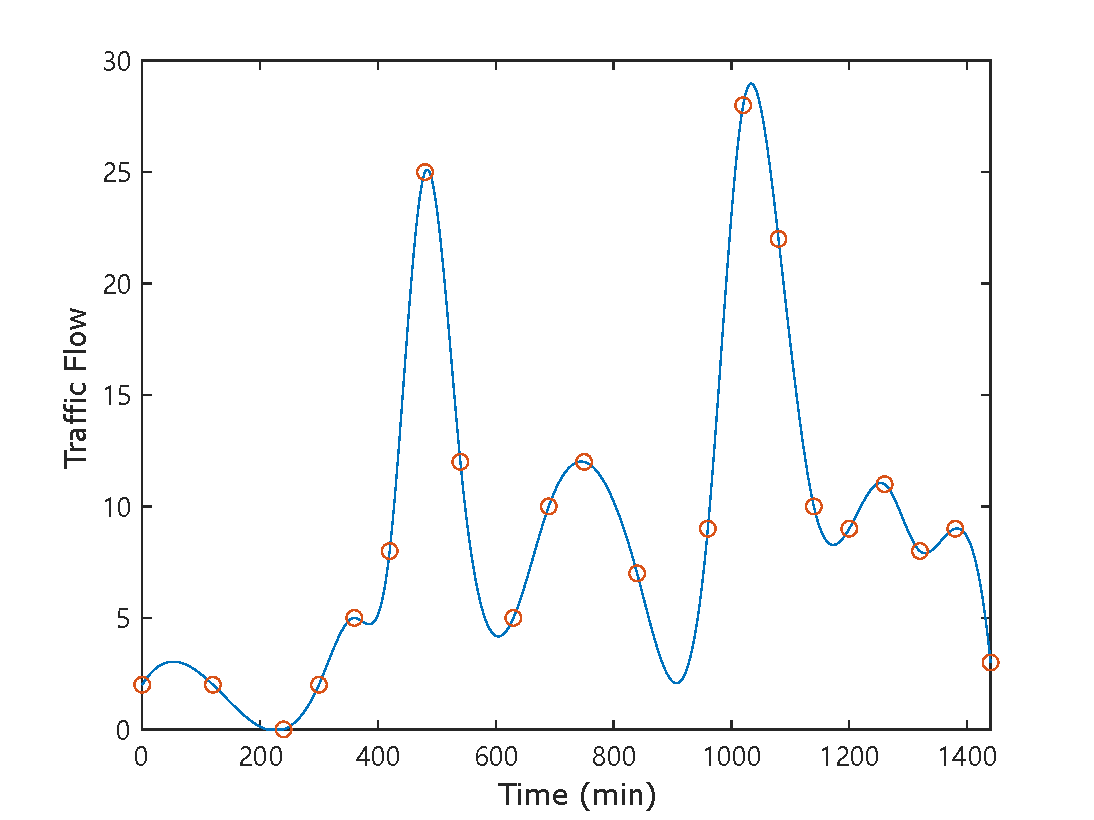
\includegraphics[width=\textwidth]{fig/ex12_spline.pdf}
    \caption{车流量曲线的三次样条插值结果}
    \label{fig:ex12_spline}
\end{figure}

\subsubsection{结果的数学分析及实际意义}

从\Cref{fig:ex12_spline}可以看出,相比于分段线性插值,三次样条插值处理后的数据更贴近真实情况,在实际生活中,车流量不会突变,车流量的变化量也往往是连续的。经过插值处理后,再通过积分算法,即可较为可靠地求出一天内的总车流量,结果约为1.27万辆。

\subsubsection{结论}

一天通过桥梁的车流量大约为1.27万辆。

\section{收获与建议}

在本次实验中,我通过使用Matlab,掌握了拉格朗日、分段线性、三次样条三种插值算法,以及梯形公式、辛普森公式、Gauss-Lobatto公式三种数值积分算法,在解决实际问题的过程中,我对数学方法的原理和应用有了更深刻的理解。

希望助教能对每次的实验进行详细的解答,希望老师在未来的课堂上介绍更多数学应用的前沿知识。

\end{document}
